\documentclass[12pt]{article}
\usepackage{graphicx} % Required for inserting images
\usepackage[a4paper, top=2.5cm, bottom=2.5cm, left=2.5cm, right=2.5cm]{geometry}

\usepackage{parskip}
\usepackage{float}
% \usepackage{ragged2e}
\usepackage{rotating}
\usepackage{multirow}
\usepackage{tabularx}
\usepackage{lscape}
\graphicspath{Thesis-report/Figures/}
\usepackage{array}
\usepackage{eso-pic,xcolor}
\usepackage{longtable}
\usepackage{booktabs}
\usepackage{array}
\usepackage{wrapfig}
\usepackage{changepage}
\usepackage{enumitem}
\usepackage{amsmath, amssymb}
\usepackage[colorlinks=true,linkcolor=blue]{hyperref}
\newcommand\AtPageUpperRight[1]{\AtPageUpperLeft{
   \makebox[\paperwidth][r]{#1}}}
   
\usepackage[english]{babel}
\usepackage{csquotes}
\usepackage[backend=bibtex,style=numeric]{biblatex}
\usepackage{setspace}
% \usepackage{natbib}

\doublespacing 
\addbibresource{references.bib}
\begin{document}
%%%%%%%%%%%%%%%%%%%%%%%%%%%%%%%%%%%%%%%%%%%%%%%%%%%%%%%%%%%%%%%%%%%%%%%%%%%%%%%%%%%%%
\begin{titlepage}
  \centering
  \vspace*{-2cm} % move the image up if needed
  
\includegraphics[width=8cm]{Thesis-report/Figures/th-deggendorf.png}
  
  \vspace{1cm}
  
  \textbf{Master Thesis}[0.5em]
  {\normalfont\fontsize{14}{16}\selectfont}
  
  \vspace{0.7cm}
  
  Deggendorf Institute of Technology, Deggendorf\\[0.5em]
  Faculty of Mechanical and Mechatronics Engineering\\[0.5em]
  Master Mechatronics and Cyberphysical Systems
  
  \vspace{4cm}
  
  {\large Objektverfolgung mit 3D‑Machine‑Vision‑Kamera für Industrieroboter}[0.5em]
  \textbf{Object Tracking using 3D Machine Vision Camera for Industrial Robots}
  
  \vspace{1cm}
  
  Master Thesis to obtain Academic Degree\\[0.5em]
  \textbf{Master of Engineering (M.Eng)}
  
  \vspace{1.5cm}
  
  submitted by: Midhun Eldose, 22101196\\[0.5em]
  first examiner: Mr. Ginu Paul Alunkal
  
  \vspace{1.5cm}

  Deggendorf, 31.07.2025
\end{titlepage}
%%%%%%%%%%%%%%%%%%%%%%%%%%%%%%%%%%%%%%%%%%%%%%%%%%%%%%%%%%%%%%%%%%%%%%%%%%%%%%%%%%%%%
%========================
% Second title page
%========================
\begin{titlepage}
  \centering
  \vspace*{1cm}
  
  \textbf{Confidential Disclosure Agreement}[0.5em]
  {\normalfont\fontsize{14}{16}\selectfont}
  
  \vspace{1cm}
  
  between\\[0.5em]
  \textbf{Deggendorf Institute of Technology}[0.2em]
  Campus Deggendorf\\
  Dieter‑Görlitz‑Platz 1, 94469 Deggendorf
  
  \vspace{1cm}
  
  Faculty of Mechanical Engineering and Mechatronics\\[0.2em]
  Major: Mechatronics and Cyberphysical Systems
  
  \vspace{1cm}
  
  Mr. Ginu Paul Alunkal\\[0.5em]
  (in the following “Deggendorf Institute of Technology”)
  
  \vspace{1cm}
  
  and\\[0.5em]
  Midhun Eldose\\[0.5em]
  (in the following “NEURA Robotics GmbH”)
  
  \vspace{1cm}
  
  (singularly and jointly “Contractual Partner”)
  
  \vspace{2cm}
  
  \textbf{Preamble}[0.5em]
  The Deggendorf Institute of Technology supervises an examination paper with the topic\\
  \vspace{1cm}
  \textbf{Object Tracking using 3D Machine Vision Camera for Industrial Robots},
   \vspace{1cm}
  \\in which,
  among other things, confidential information of the company is processed. Simultaneously,
  confidential information was also shared with the company in the context of supervision
  by the Deggendorf Institute of Technology.
\end{titlepage}

\linespread{1.5}

\textbf{Declaration}
\vspace{0.5cm}
\mbox{Name of the Student: Midhun Eldose}
\vspace{0.5cm}
\mbox{Name of the first Examiner:  Mr. Ginu Paul Alunkal }
\vspace{1 cm}
\mbox{Title of master thesis:}
\vspace{0.5 cm}
Object Tracking using 3D Machine Vision Camera for Industrial Robots
\vspace{1.5 cm}
 I hereby declare that I have written this thesis independently. I have not submitted it for any other examination purposes. I have not used other references or materials than those mentioned in the bibliography, and I have marked all literal analogous citations.
 \vspace{1.5 cm}
% 
Deggendorf,31.07.2025
\hspace{4 cm}
Signature of the student:
\linespread{1.5}
\pagenumbering{arabic}
\newpage

%%%%%%%%%%%%%%%%%%%%%%%%%%%%%%%%%%%%%%%%%%%%%%%%%%%%%%%%%%%%%%%%%%%%%%%%%%%%%%%%%%%%%
\tableofcontents
\newpage
\listoffigures
\addcontentsline{toc}{section}{List of Figures}
\newpage
\listoftables
\addcontentsline{toc}{section}{List of Tables}
\newpage

\newpage

\addcontentsline{toc}{section}{Acknowledgement}
\begin{center}
    \textbf{Acknowledgement}
\end{center}
    

    I am highly indebted to NEURA Robotics GmbH, Metzingen, for their guidance and constant supervision, as well as for providing necessary information and resources for the Master's thesis and for the support in completing the report

    \vspace{1cm}
    
    I express my special gratitude to Dr.Sugeeth Gopinathan (Head of Software Strategy), Dr.Phuong Nguyen (Software Application Expert), Mr. Norman Kohler (Senior Robotics Engineer), Mr. Amarnath Reddy Bana (Group Lead), and Mr. Florian Schnös (ProduktManager Software) for instructing, providing information about how tasks are to be done and the flow of work, and guiding me for the thesis. In addition to that, I also thank all the members for their guidance and keen support at various stages of my thesis.

    \vspace{1cm}

    I am very grateful to my academic guide, Mr. Ginu Paul Alunkal, for his full support and encouragement. I owe him for his timely guidance, suggestions, and very constructive criticism, which contributed immensely to the evolution of my thesis.
    
    \vspace{1.5 cm}
    
    
    Midhun Eldose


%%%%%%%%%%%%%%%%%%%%%%%%%%%%%%%%%%%%%%%%%%%%%%%%%%%%%%%%%%%%%%%%%%%%%%%%%%%%%%%%%%%%%
\newpage
\begin{abstract}
The tracking of the conveyor using collaborative robots equipped with vision cameras represents a significant advancement in modern production. This innovative approach enables robots to dynamically interact with moving goods on conveyor belts, enhancing efficiency, precision, and adaptability. Using vision cameras, cobots can accurately detect, locate, and track objects in real-time, accommodating changes in shape, speed, and orientation. With the incorporation of vision technology, robots can now perform tasks such as sorting, assembling, and pick-and-place operations with minimal human assistance. This thesis examines the technical aspects of cobot conveyor tracking, emphasizing the role of vision systems in enhancing automation capabilities, reducing error rates, and facilitating flexible manufacturing environ-ments. The work involves establishing a collaborative environment using cobots for conveyor tracking experiments, which utilizes a vision camera. The primary objective is to enhance the tracking accuracy of objects and capture various shapes on the conveyor belt. The setup includes a cobot, a conveyor belt, one gripper, and an object to be picked up. As the conveyor belt moves these objects, the vision camera captures their images and poses, along with their part coordinate system (PCS). The robot then synchronizes with the objects in a designated capture zone, picking them up and placing them into user-defined locations. 
\end{abstract}
\newpage
%%%%%%%%%%%%%%%%%%%%%%%%%%%%%%%%%%%%%%%%%%%%%%%%%%%%%%%%%%%%%%%%%%%%%%%%%%%%%%%%%%%%%
\section{Introduction}
\label{introduction}

In industrial robot applications, conveyor belt tracking is an essential component of robot manipulators.  As the target progresses down the production line, the task becomes increasingly complex. Robots must be aware of an object's position, orientation, velocity, size, and other characteristics.  Applications in the fields of biology, engineering, education, manufacturing, medicine, and the military all use vision sensors to identify objects.  A robot must be able to track, rearrange, and repair positioning mistakes of things on a conveyor belt when assembling electric parts into a finished product.  This information can be quickly interpreted by the visual sensor \cite{ref12}.\\

Face tracking, color tracking, and object tracking are just a few of the various engineering applications that have recently made use of tracking video.  In the industrial sector, it was used to track items such as goods, factory workers, and clothing manufacturing.  Object detection techniques and image processing for monocular video are the foundation of video tracking \cite{ref12}.\\

A vast array of tasks may be carried out by autonomous robots thanks to intelligent sensing systems.The camera is the most often used sensor in the perception system because of its low cost and large data capacity. RGB and depth cameras are the two primary categories into which camera sensors fall.  RGB and depth cameras are the two primary categories into which camera sensors fall.  RGB can only gather information about the appearance of the surrounding area; depth cameras can gather both texture and depth information at the same time \cite{ref12}.\\

The three types of depth cameras are binocular stereo depth cameras, time of flight (TOF) cameras, and structured light cameras.Structured light camera technology is quite mature, with excellent accuracy but a restricted measuring range; binocular stereo cameras are inexpensive but highly influenced by the surroundings; and TOF measurement distance is long, ideal for dynamic situations.  Structured light cameras have a two to three-meter range, but given the wealth of environmental data that can be gathered within this range, this is adequate. Due to its excellent accuracy and great range, Lidar is another sensor that is frequently used in intelligent perception systems.  Since the surroundings have less impact on LiDAR's point cloud, robot perception systems frequently use it\cite{ref12}.\\

Numerous methods have been investigated in the study of vision-driven conveyor tracking.  Real-time operation is difficult with template-matching and model-based appr-oaches because they involve complex computations and require prior knowledge of object geometry.  Motion estimates can be obtained using Kalman-filter frameworks and optical flow, but they frequently falter when backdrop textures create noise or when several objects have identical velocities.  While color-segmentation techniques are faster, they are less effective in low-contrast or monochromatic environments.  When conveyor backgrounds are relatively constant, the differential-image method—which subtracts sequential frames to identify moving regions—emerges as a convincing compromise, successfully suppressing static background and lowering computing complexity\cite{ref12}.\\

The goal of the current thesis is to expand upon and thoroughly assess this framework.  Our goals are to: (1) apply the differential-image conveyor-tracking technique in a modern robotic setting; (2) improve robustness against changing lighting and background motion by using adaptive thresholding and background modeling; (3) incorporate depth estimation using stereo or structured-light sensing to increase the accuracy of interception; and (4) carry out experimental tests evaluating performance metrics, including tracking latency, positional error, and throughput, against reference optical-flow and template-matching systems\cite{ref12}.\\

Building on this realization, Shin et al. (2006) created an eye-in-hand vision system that uses TCP/IP to communicate with a real-time robot controller and mounts a camera directly on the robot's end-effector.  The system computes centroid positions and velocities, predicts future intercept sites for the robot gripper, and accomplishes fast object detection by concentrating processing only on the regions highlighted by frame differencing.  Invoking image-processing operations, such as thresholding, binary conversion, and region labeling, is made easier by a custom "vision language" that includes command sets like VINIT, VPIC, VCOM, VTRA, and VOUT. It also reduces command complexity and makes it easier to integrate with various vision libraries\cite{ref12}.\\


In industrial production, the vision system is typically used to inspect the product.  It speeds up product detection and cuts down on time.  It is made up of a camera or vision sensor that uses line or area sensors to send digital images or videos to the host computer.  The digital image or video is analyzed using an image processing technique that allows it to identify defects, shapes, or colors.  Analysis filters are frequently used to differentiate between vision system functions such as edge detection, surface defect identification, and light intensity reflected from the product surface.  Compared to image processing algorithms, video processing algorithms are more complex \cite{ref12}.\\

A robot's job in robotic conveyor tracking is to follow and retrieve goods from a conveyor belt. Robots require information about an object, like its position, orientation, velocity, size, and other characteristics, before they can take it from an automation line. Compared to ultrasonic and infrared sensors, vision sensors are able to provide more information about an object on the conveyor belts. Typically, an object tracking system includes the following steps: taking a picture, recognizing an object, and getting information about the object's orientation and position.. A conveyor system's item tracking procedure needs to be quick enough to accommodate a real-time setting. This article describes a tracking system for robots that makes use of vision data that is taken from consecutive frames of images\cite{ref12}.\\

Many applications in the domains of construction, manufacturing, and vehicle automation and autonomy require access to 3D data. In addition to intensity, ToF (Time-of-Flight) sensors are getting more widely accessible and less expensive.. These sensors also provide depth information at each pixel.Tasks that are repetitive, dangerous, and challenging for humans to handle are frequently performed by industrial robots. Therefore, increasing the production efficiency of industrial robot manipulators is a top priority. By focusing on localisation and calculating the shortest path, image processing and path planning approaches can achieve this goal.  

This is especially crucial for the manufacturing and bottle-filling sectors, which heavily rely on robotic manipulators to position and move bottles both during production and after refills. Robot vision finds it extremely difficult to focus on distinguishing aspects of soft, fragile, or opaque things, making detection considerably more difficult. Many industrial robots and robotic manipulators have become increasingly complex, diverse, and particularly engineered to attain a high degree of autonomy. Furthermore, to provide accurate control mechanisms, object detection and tracking for these robotic manipulators have drawn a lot of interest\cite{ref2, ref12}.

Automated object detection, in particular, has helped robots become more versatile by enabling more generalized and adaptive behavior for various objects and situations. For example, DoF is important for jobs involving pick and place, welding, pelleting, painting, packing, and grinding.The DoF is chosen based on the type of work that must be done in an industrial setting and ranges from 1 to 6 degrees of freedom.Furthermore, deep learning and neural network-based methods are growing in popularity, but care must be taken with regard to these models' explainability and generalizability\cite{ref12}.\\


The three primary aspects of this work on vision-based automatic pick-and-place systems are \cite{ref12}:
\begin{enumerate}
  \item \textbf{Object Recognition}
  \item \textbf{Machine Vision System Calibration}
  \item \textbf{Object Coordinate Transformations}
\end{enumerate}

The calibration of the machine vision system is further composed of three components \cite{ref12}:
\begin{itemize}
  \item \textbf{Hand–Eye Calibration}
  \item \textbf{Stereo Calibration}
  \item \textbf{Camera Calibration}
\end{itemize}

This study computes the transformation link between the camera coordinate system (``eye'') and the robot base coordinate system (``hand'') using homogeneous transformation matrices for hand–eye calibration\cite{ref12}.

Identifying objects in an image and determining their positions is the primary goal of object recognition. Four steps are typically involved in 3D object identification \cite{ref12}:
\begin{enumerate}
  \item Interest‑Point Detection \cite{ref12}
  \item Interest‑Point Description \cite{ref12}
  \item Match‑Point Error Elimination \cite{ref12}
  \item Model Recognition and Pose Estimation \cite{ref12}
\end{enumerate}
It is more difficult for robotic arms to do complex operations like object pick-and-place independently.  Integrating machine vision into the robotic arm system is one potential remedy for the issues previously highlighted. This research uses the eye-to-hand camera arrangement to construct vision-based autonomous pick-and-place systems for 3-D objects. Object coordinate transformations, machine vision system calibration, and object identi-fication are the three main parts of the vision-based autonomous pick-and-place system developed in this study.   Experimental results show that the vision-based automated pick-and-place system developed in this study can perform an autonomous pick-and-place job for 3-D objects\cite{ref12}.
\newpage

%%%%%%%%%%%%%%%%%%%%%%%%%%%%%%%%%%%%%%%%%%%%%%%%%%%%%%%%%%%%%%%%%%%%%%%%%%%%%%%%%%%%%
\section{Literature Review}
\subsection{Robotic Conveyor Tracking}
Early work on visually guided conveyor tracking focused on 2D cameras and simple background-subtraction methods\cite{ref12} demonstrated frame-difference object detection com-bined with 2D template matching to locate parts on a belt in real time, but had issues with homogeneous lighting and occlusion.\cite{ref14} formulated the conveyor-tracking problem as a constrained trajectory‐planning task for 6-DOF manipulators, minimizing steady-state tracking error and actuator torques: More recently,\cite{ref9} integrated time-of-flight ranging with color segmentation to classify and track parcels at higher belt speeds, achieving sub-5 mm positional accuracy at 1 m/s.\\

\subsection{3D Vision Systems and Depth Sensing}
The shift from 2D to 3D sensing has been driven by affordable structured light and ToF cameras\cite{ref2}. Photoneo’s MotionCam 3D M+ uses Parallel Structured Light to capture 1068 × 800 depth frames at 60 Hz, merging per-pixel depth with intensity for robust object detection under ambient light. \cite{ref17} showed how ToF depth data can be converted from spherical to Cartesian coordinates for conveyor-based pick-and-place, with typical z-noise under 0.5 mm at 1 m distance.\ \cite{ref3} extended this by fusing stereo vision point clouds with ToF to improve tracking through partial occlusions.\\


\subsection{Calibration Techniques (Hand–Eye and Extrinsic)}
\cite{ref3} describes that accurate hand-eye and extrinsic calibration are critical for mapping camera coordinates into the robot base frame. Standard methods use a calibration rig (ball or checkerboard) and solve for the transform ${}^{\rm base}H_{\rm cam}$ via least‐squares on multiple correspondences\cite{ref2}.Photoneo-automated lidar–camera extrinsic calibration with a hemi-spherical target, yielding sub‐millimeter accuracy over nine poses, and Photoneo’s web interface further streamlines extrinsic setup by guiding users through nine sample points and reporting an overall accuracy score in millimeters.

\subsection{Dynamic Object Tracking and Path Planning} \cite{ref1} describes real-time tracking of moving parts, which requires coupling image processing updates with trajectory replanning, and proposes an image processing‐based path planning system in which each new depth image triggers local replanning via a fast pseudo‐inverse Jacobian update that ensures collision‐free smooth motion.\cite{ref4} introduced dynamic treatment of occlusion in 3D by predicting object position through Kalman filtering of multi‐view point clouds.\cite{ref7} Demonstration of shadow casting to improve grip edges, reducing processing latency in high‐speed pick‐and‐place.

\subsection{Gaps and Research Directions}
Despite these advances, challenges remain in  
\begin{itemize}[nosep]
  \item \textbf{High‐speed tracking:} maintaining sub-millimeter accuracy above 1 m/s belt speeds.
  \item \textbf{Dynamic lighting:} achieving robust detection under rapidly changing ambient conditions.
  \item \textbf{Transparent/reflective objects:} current depth sensors struggle with non-Lambertian surfaces.
  \item \textbf{Explainability and safety:} integrating uncertainty estimates into real‐time safety controllers.
\end{itemize}


\newpage
\section{Working Principle}
\subsection{Euler Angles}
Euler angles are one method of parameterizing the space of alignments.  A global orientation can be expressed as a sequence of rotations along three mutually orthogonal axes in space using Euler angles.

To solve differential equations, Euler initially created Euler angles. The most popular technique for parameterizing the space of orientations is now the use of Euler angles. If we choose to consider a rotation as the action performed to attain a particular orientation, we can use Euler angles to parameterize the space of rotations\cite{ref20}.

\subsection{Disadvantages of Gimbal Lock and Ambiguity}
\subsubsection{Gimbal Lock}
\begin{itemize}
  \item \textbf{Loss of One Degree of Freedom.} 
   One ``gimbal'' loses its capacity to rotate on its own when two of the three rotation axes align (for instance, the X' axis aligns with Z in a Z–X'–Z sequence).  As a result, the three-dimensional local parameter space shrinks to two dimensions\cite{ref20}.
  \item \textbf{Numerical Instability.} 
    Small orientation changes necessitate huge swings in two of the Euler angles, which amplifies floating-point mistakes, especially near the unique alignment (e.g., a pitch of $\pm90^\circ$ in a Z–Y'–X sequence)\cite{ref20}.
  \item \textbf{Control \& Interpolation Problems.} 
    Smoothly interpolating through a gimbal-lock singularity might result in abrupt flips or unpredictable motion in applications like animation or flight control\cite{ref20}.
\end{itemize}

\subsubsection{Ambiguity (Non-Uniqueness)}
\begin{itemize}
  \item \textbf{Multiple Angle Triples for the Same Rotation.} 
   There are an unlimited number of those \((\alpha,\beta,\gamma)\) that produce the same rotation matrix since every rotation about an axis is periodic (modulo \(360^\circ\)) and because different sequences might arrive at the same ultimate orientation\cite{ref20}.
  \item \textbf{Convention Dependence.} 
    There are twelve main Euler conventions, including choice of axis ordering, intrinsic vs. extrinsic, and proper Euler vs. Tait–Bryan.  In the absence of precise convention, a \((\alpha,\beta,\gamma)\) triplet is unclear\cite{ref20}.
  \item \textbf{Inverse-Mapping Ambiguities.} 
   Solving for Euler angles given a rotation matrix frequently produces two valid answers (referred to as the "standard" and "suppl-ementary" sets), necessitating additional reasoning to select one\cite{ref20}.
\end{itemize}

\subsubsection*{Why It Matters}
\begin{itemize}
  \item \textbf{Robustness:} Systems like VR head-tracking, robotic manipulators, and airplane autopilots can all be rendered inoperable by gimbal lock\cite{ref20}.
  \item \textbf{Maintainability:} To prevent misunderstandings, ambiguity compels programs, file formats, and APIs to explicitly state which Euler standard is being used\cite{ref20}.
\end{itemize}

\subsubsection*{Alternatives}
Many applications prefer other orientation representations to avoid both gimbal lock and ambiguity:
\begin{itemize}
  \item \textbf{Quaternions.}  It is unique up to a sign, free of singularities, and provides smooth spherical linear interpolation (slerp)\cite{ref20}. 
  \item \textbf{Rotation Vectors/Axis-Angle.}  One-to-one mapping (except for periodicity and sign and \(2\pi\) \cite{ref20}. 
  \item \textbf{Rotation Matrices.}  Despite being over-parameterized (9 integers with 6 restrictions), it is clear and globally non-singular\cite{ref20}. 
\end{itemize}

\subsubsection{Rotation matrices}
Euler angles are usually implemented using rotation matrices. There is an x rotation matrix, a y rotation matrix, and a z rotation matrix for every kind of roll. The matrices are multiplied by the position vector for a point in space to generate the position vector for the rotated point.  Despite being a 3 × 3 matrix, a rotation matrix is usually replaced by a homogeneous 4 × 4 matrix. The three roll matrices corresponding to the three Euler angles are multiplied to produce a general rotation. The generated matrix can be applied to the locations that need to be rotated and represents the general rotation. In most cases, matrix multiplication is not commutative.This is consistent with rotations in space not commuting.
 Lastly, it should be mentioned that the only way to effectively incorporate all common
transformations, such as translation, scaling, shearing, and different projections
transformations, is to use homogeneous transformation matrices\cite{ref20}.

\subsection{Quaternions}
The second rotational modality uses quaternions and is defined by Euler's theorem. Since there isn't a thorough introduction to the subject and quaternions aren't nearly as well-known as transformation matrices, we will give a brief history before going into great detail into quaternion mathematics.\cite{ref20}.\\

\subsubsection{Rotations and Euler’s Theorem}
Rotations in 3D can be implemented using Euler’s theorem combined with quaternions, an extension of complex numbers\cite{ref20}.

\subsubsection{Impossibility of 3D ``Complex'' Numbers}
The following equation are taken from \cite{ref20}
Hamilton originally attempted to define three-dimensional complex numbers of the form\\
\[
  a + i\,b + j\,c,\quad i^2 = j^2 = -1,
\]
closed under multiplication. Jones Kenneth\cite{jones1984kenneth} showed by contradiction that no such 3D system exists:
\[
  \text{Assume }i\,j = a + i\,b + j\,c,\quad
  i^2 = j^2 = -1.
\]
A brief outline of the contradiction leads to
\[
  c^2 + 1 = 0,\quad c\in\mathbb{R},
\]
which is impossible.

\subsubsection{Hamilton’s Discovery of Quaternions}
Hamilton discovered that four elements are required to depict a rotation followed by scaling in three dimensions while strolling by Dublin's Royal Canal: \cite{ref20}
\[
  q = s + x\,i + y\,j + z\,k,
  \quad
  i^2 = j^2 = k^2 = ijk = -1.
\]
Here:
\begin{itemize}
  \item $s\in\mathbb{R}$ is the \emph{scalar part} (encoding uniform scaling).
  \item $\mathbf{v} = (x,y,z)\in\mathbb{R}^3$ is the \emph{vector part} (encoding rotation axis and angle).
\end{itemize}

\subsubsection{Quaternion Notation}
We often write a quaternion as
\[
  q = [\,s,\;\mathbf{v}\,],\quad s\in\mathbb{R},\;\mathbf{v}\in\mathbb{R}^3.
\]
This four-dimensional algebra provides a compact, non-singular representation of 3D rotations.

\subsection{Inverse Kinematics}
The system model includes a non-redundant robot manipulator with n degrees of freedom and a conveyor belt system. The following attributes are assumed to be present in the system model: \cite{ref14}
1) The conveyor belt system runs at constant velocity, and the
part is stationary relative to the conveyor belt system\cite{ref14}.\\
2) The orientation of the robot hand is initially aligned with the part and kept fixed while the robot tracks the part\cite{ref14}.\\
3) The robot tracks the part along a straight path over the
conveyor belt system \cite{ref14}.

\begin{figure}[h]
    \centering
    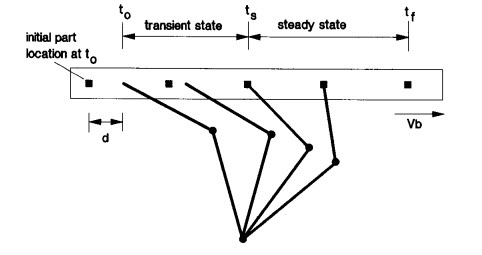
\includegraphics[width=9cm]{Thesis-report/Figures/ik.jpeg}  
    \caption{Kinematics \cite{ref14}}
    \label{fig1.Photoneo Cmaera}
\end{figure}

Robot motion must meet certain conditions to maximize the usable performance of the manipulator on conveyor tracks, including \cite{ref14}:

1) \textbf{Steady-state error:}  The task's accuracy may be reduced due to location and velocity errors in the steady state. Therefore, the steady-state error in the conveyor tracking trajectory must be as low as possible \cite{ref14}.\\\\
2)  \textbf{Constraints on torque and smoothness:}The trajectory must be created so that all joint torques remain within their ranges at all times\cite{ref14}.\\\\
3) \textbf{Settling time:}  Settling time: The time needed for the task gets less as the robot quickly reaches a steady state.The robot's torque and smoothness restrictions, the conveyor belt speed, and the initial positions of the robot and the part should all be considered for minimizing the settling time\cite{ref14}.\\\\
The joint variables in the forward kinematics issue establish the end-effector's position and orientation in Cartesian space, also known as the workspace. The link extensions for prismatic joints and the angles between the links for rotational joints are the joint variables. Finding the values of the joint variables that allow the manipulator to reach the designated location, given a desired end-effector position and orientation, is the challenge of inverse kinematics.  Figure 2 below shows the connection between joint space, Cartesian space, and forward and inverse kinematics\cite{ref10}.\\

\begin{figure}[h]
    \centering
    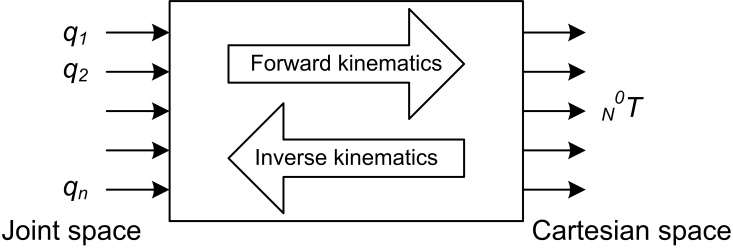
\includegraphics[width=12cm]{Thesis-report/Figures/fk.png}  
    \caption{Forward and Inverse Kinematics \cite{ref10}}
    \label{fig:inverse-kinematics}
\end{figure}

Finding the joint variables that allow a robot to be manipulated into the required position requires an understanding of its inverse kinematics. This is used to control the robot's position, motion, and other features. This study presents a detailed explanation and comparison of two popular approaches for manipulating robots: Jacobian inverse techniques and inverse kinematics.Sixteen alternatives are available for a general six-DOF robot, as shown below, and they list the number of analytical solutions for robots with varying degrees of freedom. Consequently, a precise set of answers among several inverse kinematic solutions is needed for a robot to move constantly\cite{ref10}.\\


The benefit of analytical expression is that it provides formulas for the connection between link parameters and joint angles. The robotics controller can directly incorporate these relationships\cite{ref10}.\\

\begin{table}[h]
    \centering
    \begin{tabular}{cc}
        \toprule
        \textbf{DOF} & \textbf{Number of Solutions} \\
        \midrule
        6 (6R, 5RP) & 8 \\
        6R (intersecting wrist)
Greater than 6 & 16\\
        (Redundant manipulator) & inf.\\
        \bottomrule
    \end{tabular}
    \caption{DOF vs. Number of Solutions \cite{ref19}}
    \label{tab:dof_solutions}
\end{table}
\subsection{Jacobian inverse method}
The time derivative of the kinematic equations that connect the end-effector's velocity to the joint rates is known as the Jacobian in robotics. The following is the phrase for the Jacobian \cite{ref19}.
\subsubsection{Kinematic Velocity Equations}

The following equations are taken from \cite{ref19}:\\\\
The end-effector angular and linear velocities are given by
\begin{align}
  \omega_e &= J_{\omega}(\theta)\,\dot{\theta}, \\
  v_e      &= J_{v}(\theta)\,\dot{\theta},
\end{align}
where,

\begin{description}
  \item[$\theta$]%
    Joint coordinate vector of size $n$.
    \begin{itemize}
      \item 0i is the i-th joint displacement for prismatic joints, and 0i is the i-th joint angle for revolute joints.
    \end{itemize}

  \item[$\dot{\theta}$]%
    Joint velocity vector (time derivative of $\theta$).
    \[
      \dot{\theta} = \begin{bmatrix}
        \dot{\theta}_1 \\ \dot{\theta}_2 \\ \vdots \\ \dot{\theta}_n
      \end{bmatrix},
    \] 
    with units: rad/s for revolute and m/s for prismatic joints.

  \item[$J(\theta)$]%
    Geometric Jacobian, a $6\times n$ matrix mapping $\dot\theta$ to the end-effector twist.
    \[
      J(\theta) = 
      \begin{bmatrix}
        J_v(\theta) \\[6pt]
        J_\omega(\theta)
      \end{bmatrix}.
    \]

  \item[$J_v(\theta)$]%
    Linear‐velocity submatrix of $J$. It’s the top 3 rows:
    \[
      J_v(\theta) \in \mathbb{R}^{3\times n},
      \quad
      v_e = J_v(\theta)\,\dot\theta
      \;\in\; \mathbb{R}^3.
    \]

  \item[$J_\omega(\theta)$]%
    Angular‐velocity submatrix of $J$. It’s the bottom 3 rows:
    \[
      J_\omega(\theta) \in \mathbb{R}^{3\times n},
      \quad
      \omega_e = J_\omega(\theta)\,\dot\theta
      \;\in\; \mathbb{R}^3.
    \]

  \item[$v_e$] the end‐effector linear velocity vector in the base/world frame:
    \[
      v_e = \begin{bmatrix} \dot{x} \\ \dot{y} \\ \dot{z} \end{bmatrix},
    \]

  \item[$\omega_e$]is the end‐effector angular velocity vector in the base/world frame:
    \[
      \omega_e = \begin{bmatrix} \omega_x \\ \omega_y \\ \omega_z \end{bmatrix},
    \]
\end{description}
where the $3\times6$ matrices $J_\omega$ and $J_v$ relate the joint velocities or rates $\theta$ to the end-effector velocity $v_e$ and angular velocity $\omega_e$, respectively. Note that $J_\omega$ and $J_v$ are both functions of $\theta$, denoting the relation to the robot orientation. It is possible to rewrite the end effector displacement as a function of the Jacobian $J(\theta)$ as \cite{ref19}:

  \[
    \Delta x_e = J(\theta) \, \Delta \theta 
  \]

This is a first-order Taylor expansion and is valid for small $\Delta \theta$

\subsection{Inverse Kinematics Using Jacobian}

If the Jacobian $J(\theta)$ is square and invertible (e.g., for a 6-DOF manipulator), then:\cite{ref19}

  \[
    \Delta \theta_k = J_k^{-1} \Delta x_e ,
  \]

And the joint update becomes:

  \[
    \theta_k = \theta_{k-1} + J_k^{-1} \Delta x_e  
  \]

\subsection{Redundant Manipulators and Pseudoinverse Solution}

For manipulators where $J$ is not square (e.g., redundant robots with $n > 6$), we use the Moore–Penrose pseudoinverse $J^\dagger$:\cite{ref19}

  \[
    \theta_k = \theta_{k-1} + J^\dagger \Delta x + (I - J^\dagger J)\Delta \phi 
  \]

where:
\begin{itemize}
    \item $J^\dagger$ is the pseudoinverse of $J$ \cite{ref19}. 
    \item $(I - J^\dagger J)$ projects into the null space of $J$\cite{ref19}.
    \item $\Delta \phi$ is a secondary objective function direction (e.g., for obstacle avoidance or joint limit avoidance)\cite{ref19}.
\end{itemize}

\subsection{Jacobian Construction}

Every column in the Jacobian matrix represents a joint's contribution to the motion of the end-effector: \cite{ref19}.
\begin{itemize}
    \item For a revolute joint $i$:\cite{ref19}.
    \[
        J_i = \begin{bmatrix}
            \mathbf{z}_i \times (\mathbf{o}_n - \mathbf{o}_i)\\
            \mathbf{z}_i 
        \end{bmatrix}
    \]
    \item For a prismatic joint $i$:\cite{ref19}.
    \[
        J_i = \begin{bmatrix} 
            \mathbf{z}_i \\
            \mathbf{0}
        \end{bmatrix}
    \]
\end{itemize}
where:
\begin{itemize}
    \item $\mathbf{z}_i$ is the axis of joint $i$ in base coordinates.
    \item $\mathbf{o}_i$ is the origin of frame $i$, and $\mathbf{o}_n$ is the end-effector origin.
\end{itemize}

\subsection{Robot Coordinate System} 
We must first gain a fundamental understanding of the robot coordinate system before delving deeper into the tracking system's operation. Generally speaking, robotic systems are Cartesian coordinate systems with three axes: the X, Y, and Z axes. Additionally, there is the Rotation Coordinate System, which describes the robot's degree of rotational motion and joint function. However, as this format is more widely used in business and simpler to use and comprehend, we shall solely investigate the Cartesian coordinate system. The following terms used in the system should be understood to obtain the robot's coordinates \cite{ref24}.

\subsubsection{System of World Coordinates (WCS)}
A coordinate system is often specified by the user or developer, but it can exist anywhere in the world. WCS makes it simpler to explain the locations of other things or items in that specific area. Origin placement is typically done at the edge of a group or a room's corner \cite{ref24}.\\

 \textbf{Machine Coordinate System (MCS)}
Robot Base Frame Coordinate System is another name for Machine Coordinate System (MCS). All other coordinate systems will be compared to this most significant coordinate system. Where developers and programmers would implement their code based on this coordinate system is equally crucial. For the point of origin, MCS is usually placed close to the robot's base, though it's crucial to keep in mind that different robot types have different bases \cite{ref24}.\\

 \textbf{Coordinate System for Parts and Workpieces (PCS)}
The workpiece or monitored items that move along the conveyor belt are referred to here. In certain applications, part orientation plays a crucial role in assembly procedures. In our application, we just want to choose or select the objects, independent of their orientation; thus, this isn't accurate\cite{ref24}.\\

 \textbf{Tool Coordinate System (TCS)}
 This refers to the location of the robot's end-tip. As you can see, a robotic hand typically has a mechanism attached to the end with a gripper. When referring to the robot base frame, this typically requires a small amount of offset and aids the robot in completing its responsibilities \cite{ref24}.\\\\
 \textbf{ Coordinate Transformation Matrix:}  \\
 In essence, the coordinate transformation matrix is a matrix that depicts how a coordinate system's orientation changes from one frame to another. It describes both rotation and translation transformation and is composed of a 3x3 rotation matrix and a 3x1 displacement vector.  In the case of three dimensions, the matrix is 4x4.  The homogeneous transformation matrix is a more popular and often used term for this matrix.  Keep in mind that this matrix can be used for forward kinematics calculations and standard coordinate transformation procedures, among other coordinate transformation scenarios \cite{ref24}.\\\\

\begin{figure}[h]
    \centering
    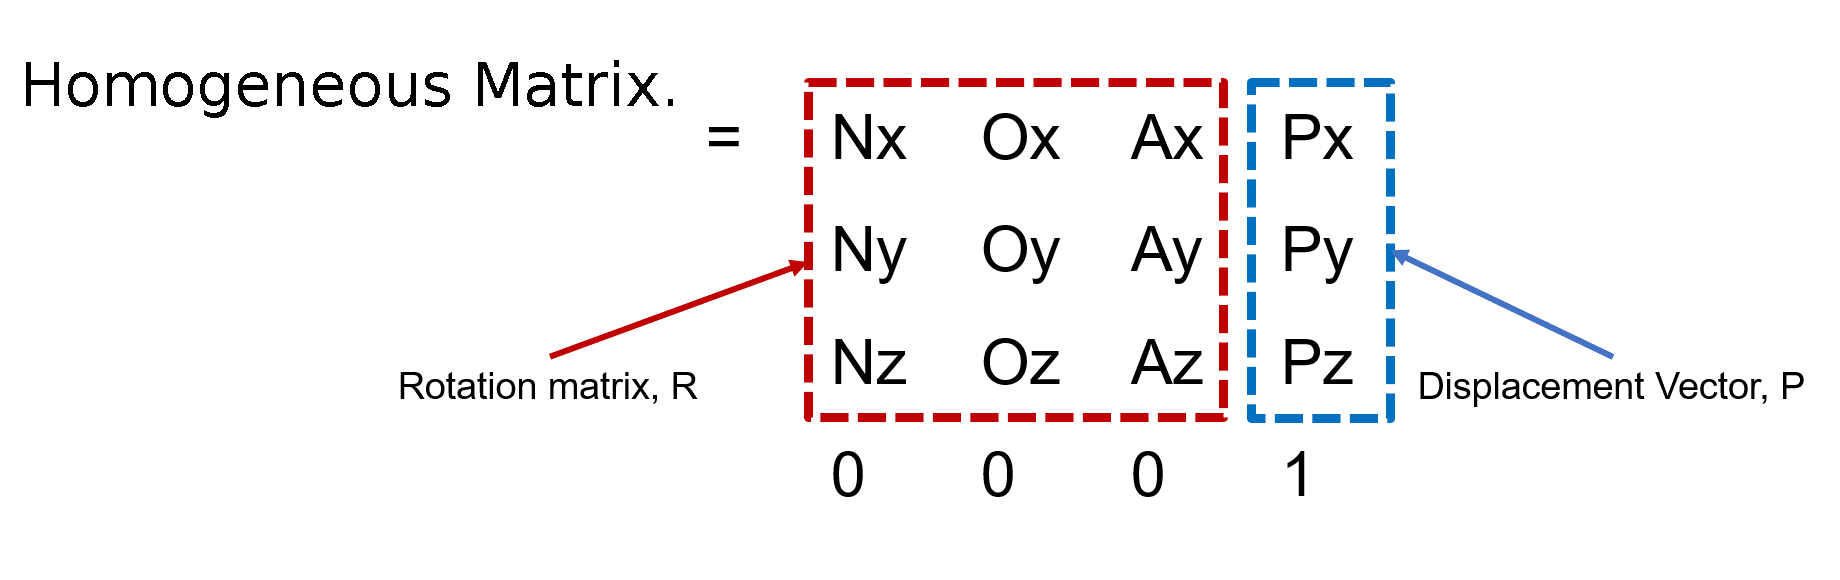
\includegraphics[width=15cm]{Thesis-report/Figures/transform.png} 
    \caption{Homogenous transform \cite{ref25}}
    \label{fig1.Photoneo_Camera}
\end{figure}
\newpage
\subsection{Working Flowchart:}
\begin{enumerate}
    \item Start
    \item Initially, check if the operation type is OBJECT POSE
    \item If not, raise a problem to demonstrate that there is an unforeseen problem.
    \item If yes: Receive object pose data
    \item Then unpack the object pose and set them as ([X,Y,Z,ex,ey,ez])
    \item Convert the first three elements to meters ([X.Y, Z])
    \item Set the velocity and timeout for picking
    \item Record the start time
    \item Calculate the current time and update the position X with the equation \[  
X = X_0 + v\,t
\]

    \item Create the target position with the quaternion values received from the camera
    \item Check the condition where the object needs to be picked; if the distance is less than 700, then do the motion of move linear ()
    \item If not successful,  break the loop and print that the target is too far
    \item Get the current joint angles and TCP pose, and calculate the distance to the object.
    \item If the distance to the object is less than 5, then send the signal to the gripper and pick the object.
    \item If the timeout to pick is greater compared to the given input, then break the loop.
\end{enumerate}
\newpage
The following figure shows the flowchart for the dynamic picking:\\
\begin{figure}[h]
    \centering
    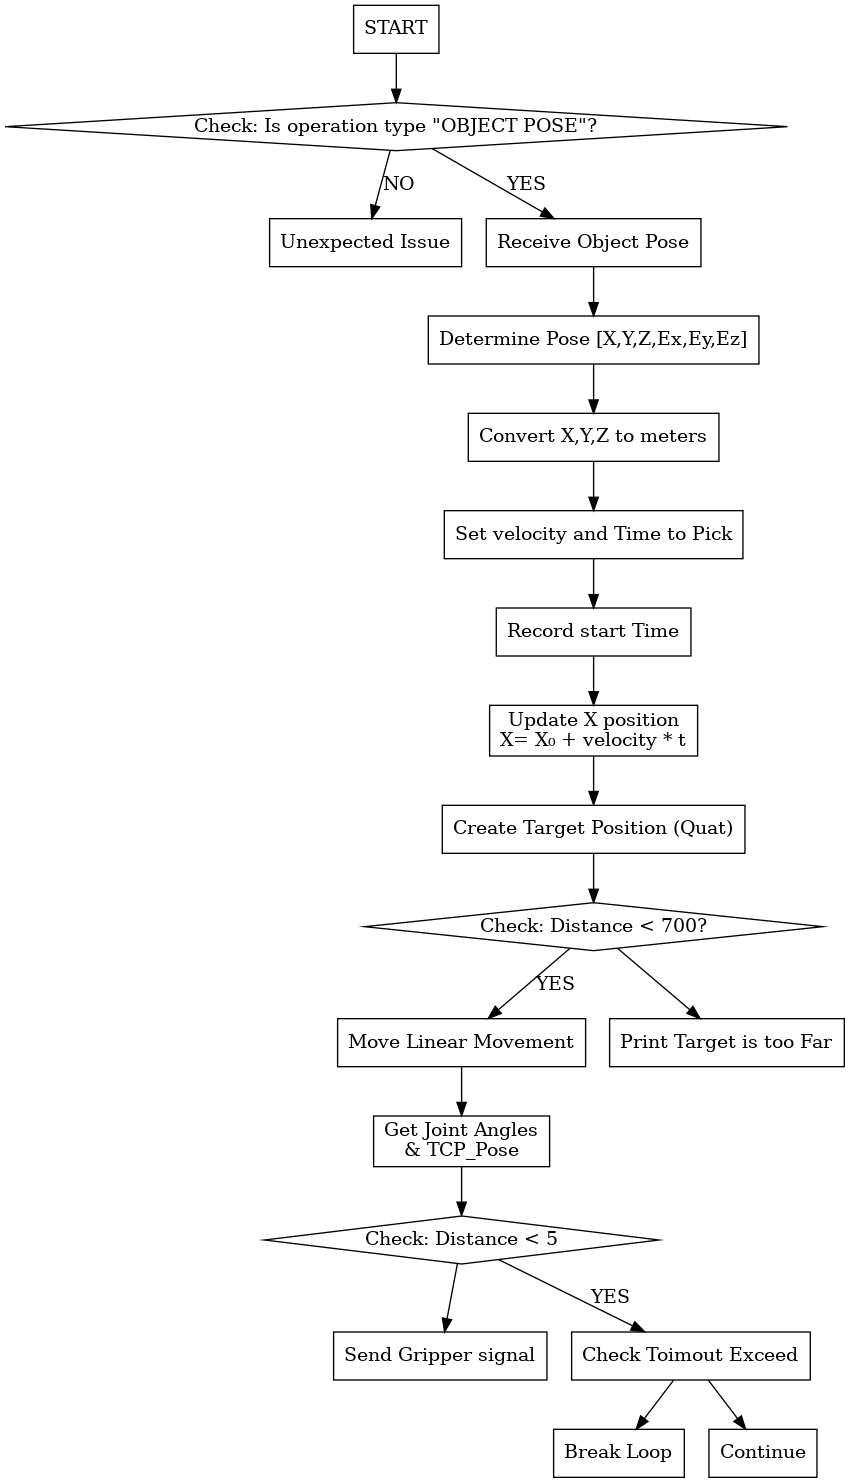
\includegraphics[width=10.3cm]{Thesis-report/Figures/flowchart.png}  
    \caption{Working Principle flowchart}
    \label{fig2.Photoneo_Cmaera}
\end{figure}
\newpage

\newpage

\subsection{Operations Needed to Develop the Tracking System}
The tracking system's pillars are composed of three primary components. Only a scenario including a camera, a belt conveyor, and a robot will be covered in this post. It is certainly possible to expand the tracking system by including additional robots and cameras. The principles will not change, even if more complex processes will be needed to account for extra elements\cite{ref25}.\\

\subsubsection{Conveyor Belt to Camera Conversion (B1)}
The orientation of the conveyor belt coordinates and the camera origin coordinates deviate from one another. The origin of a camera is the upper left corner of its field of vision (FOV), where the values of its pixels start at (0, 0). This origin is set in stone and cannot be altered. Although the origin's location for the conveyor belt can be freely specified, the normal practice is to first select the picking window's dimensions (it is square), taking into account the robot's picking range limit, and then position the origin in the middle of the bottom of the window\cite{ref25}.\\

\begin{figure}[h]
    \centering
    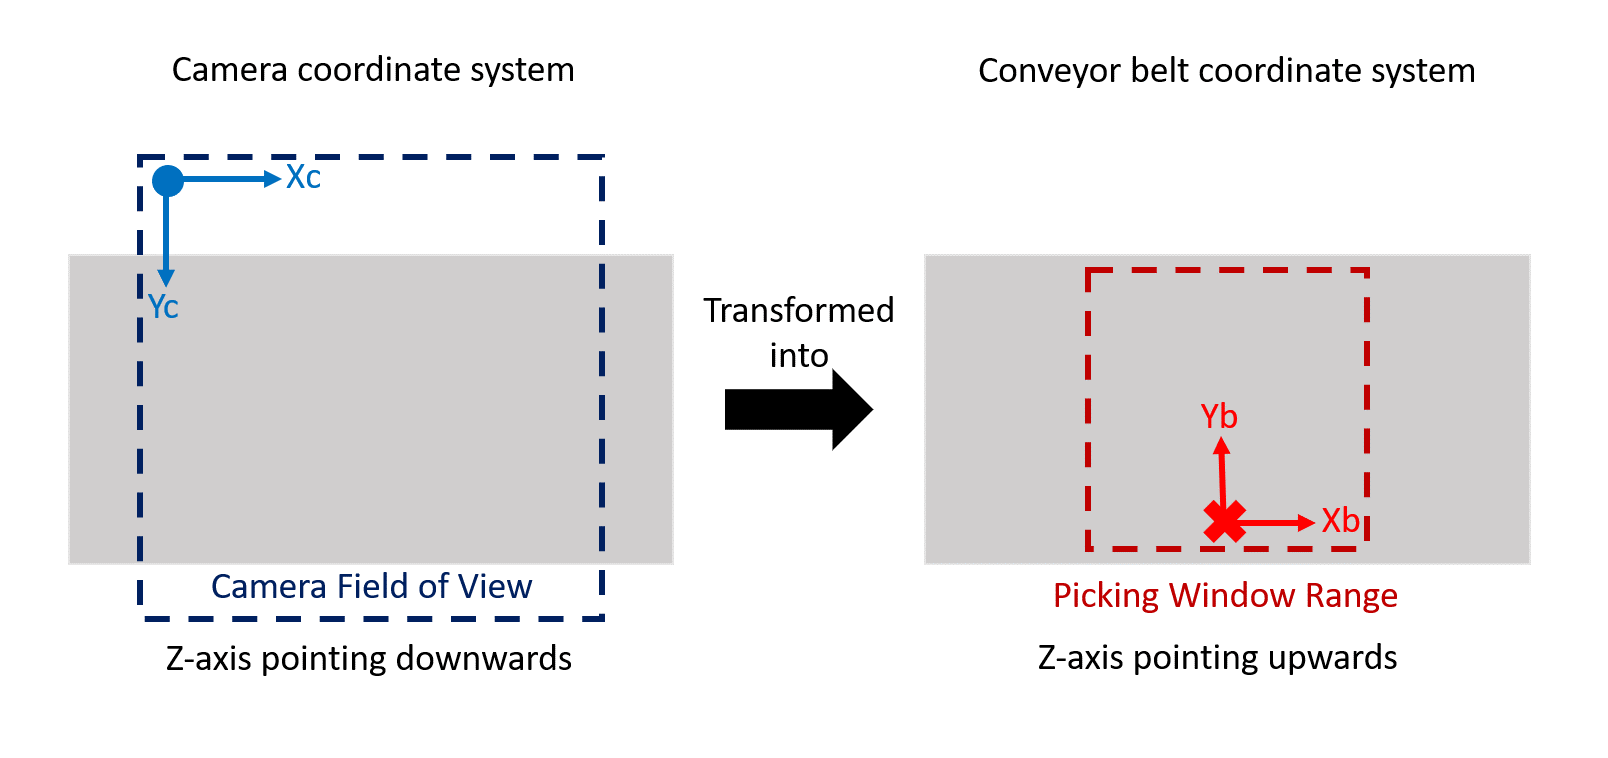
\includegraphics[width=15cm]{Thesis-report/Figures/camera to conveyor.png}
    \caption{Conveyor to camera conversion \cite{ref25}}
    \label{fig1.Photoneo Cmaera}
\end{figure}
As can be seen in the above image, to match the origin of the conveyor belt, we must perform a translation transformation on both the X and the Y axes. We must do a rotation transformation for the Z-axis, since the belt origin faces the other direction from the camera origin. In summary, this section contains two transformations: the rotation transformation, $\text{Rot}(x, 180^\circ)$, and a translation in the X-axis and Y-axis, $\text{Trans}(\Delta X, \Delta Y, 0)$. Observe that both the Y and Z axes changed their facing directions when we rotated the X axis. For this section, some offset will be required \cite {ref25}.\\

\subsubsection{Conveyor belt (B1) to conveyor belt (B2) transformation}
For this part, it is quite simple. This transformation is about the movement of the conveyor belt from the camera’s field of view to the robot’s workspace/pick range. The only value that changes in this transformation is the X-axis value. As was indicated in the beginning, we also use the encoder's reading to monitor the conveyor belt's travel distance\cite{ref25}.\\

\begin{figure}[h]
    \centering
    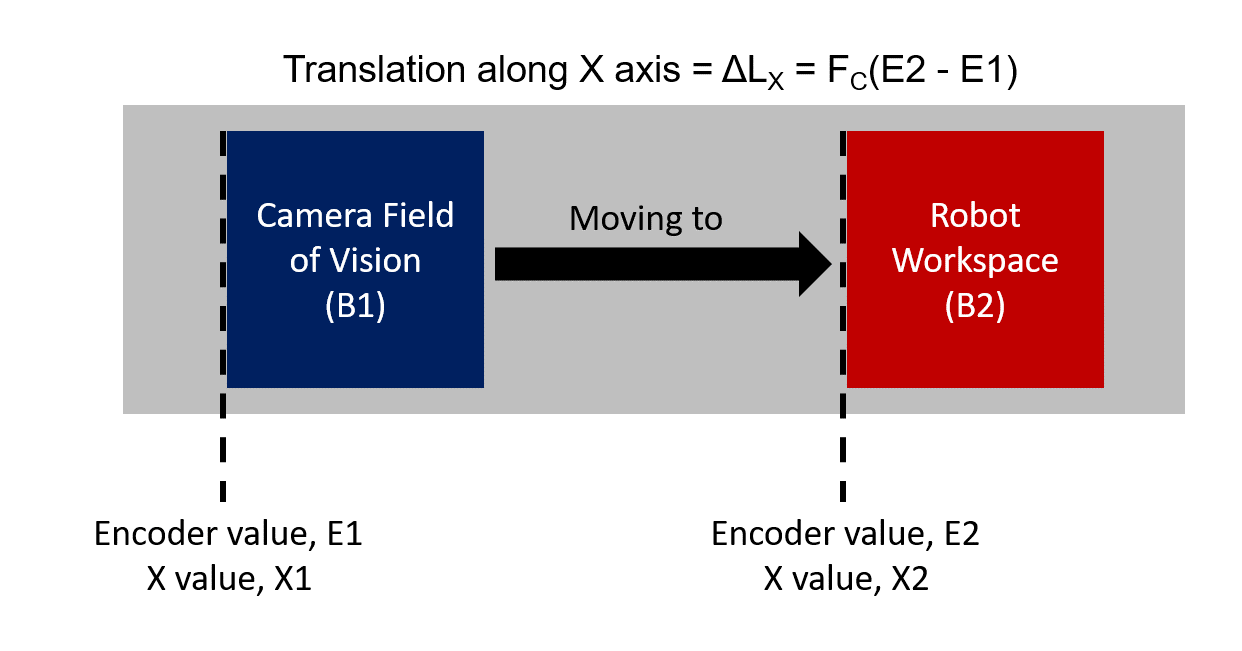
\includegraphics[width=10cm]{Thesis-report/Figures/cam to conv.png}
    \caption{Conveyor belt b1 to b2 conversion \cite{ref25}}
    \label{fig1.Photoneo Cmaera}
\end{figure}
\newpage
\subsection{Robotic Movement:}
The robotic movement can be performed with 3 methods called Servo X, Servo J, and Movelinear.\
\begin{itemize}
    \item ServoX
    \item Servo J
    \item MoveLinear
\end{itemize}
1. \textbf{ServoX:}The Servo X motion involves moving the robot in Cartesian motion, using the quaternion poses [X, Y, Z, Qx, Qy, Qz, W] as a representation of the coordinates we receive from the camera.These are already in Cartesian poses, which can be directly passed to the robotic controller, giving these values as the target position and moving the robot to the desired location. During motion, the camera coordinates were not in the correct order as those of the robotic movement, so initially, the target position had to be changed as in this form [X, Y, Z, W, Qx, Qy, Qz].\\\\
2. \textbf{ServoJ:} When using ServoJ, the robot moves with the joint movements rather than Cartesian. The object coordinates that we get from the camera are in Cartesian form; they need to be converted into joint form and given as the target position. The final orientation values of the coordinates when providing the target position will differ from the robot's TCP coordinates. To set this, we have to implement the method of inverse kinematics.\\\\
3. \textbf{Movelinear:}
With the Movelinear controller, the camera scans the objects to deliver the quaternion values, which are then used to immediately determine the target position for the robot to pick up the object. Here, we specify the top speed and acceleration.  Through a servo interface, quaternion values are sent to the robot as the target position in order to move it to the desired location.

\newpage
\subsection{Coordinate Transformation:}
The availability of 3D data is essential for numerous applications in the fields of vehicle automation ,manufacturing and autonomy.  Time-of-flight (ToF) sensors are getting cheaper and more available. They offer in-depth information for every pixel at every pixel in addition to intensity. Within its field of vision, the ToF sensor gives spherically coordinated range data about the surrounding environment. The spherical coordinates are transformed into Cartesian coordinates, as described in the following section, with the origin of the coordinate system located at the center of the camera.  With the origin at a known reference point, the 3D point cloud in the camera coordinate system is converted to the belt coordinate system. The tests examine the capacity of ToF sensors to provide sensing for a robot tasked with handling goods traveling on a conveyor belt in an indoor scenario. The range data is utilized to identify and calculate the dimensions of objects traveling along a conveyor belt.  The robot then receives the geometry and recognition data for additional action.  The findings suggest that ToF sensors have immediate potential for automating these kinds of applications \cite{ref5}.\\

 The coordinate transformation is necessary for two reasons:\cite{ref5}
 \begin{enumerate}
     \item  To enable the robot to be guided by the range camera's measurements, the robot and the camera must agree on a coordinate system\cite{ref5}.

    \item In the belt coordinate system, the z-axis is normal to the belt plane.  By referring to points above the belt plane ($z >= 0$) and inside the belt limits, this alignment of the coordinate axis makes it easier to extract item point clouds on the belt \cite{ref5}.
 \end{enumerate}
 \subsection{Robotic Motion}
Given a point in the world coordinate, the angle of each joint is calculated based on an inverse kinematics (IK) equation. In general, there may be no analytic IK solution from a manipulator for the configurations of each joint. The numerical method is introduced to solve the problem for
general manipulators. The velocity of the joint can be mapped to Cartesian space with the Jacobian linearization method\cite{ref19}.
\\

\[
v = J(q) \dot{q} 
\]

Pseudo-inverse is used to solve the joint:\cite{ref19}


\[
\dot{q} = J^\dagger \dot{x}, \quad J^\dagger = (J^T J)^{-1} J^T
\]

Velocity for the linear velocity in Cartesian space. First, FK is used to determine the manipulator's pose. Next, the IK solver uses a pseudo-inverse calculation to update the joint angles. Until the end tip reaches the desired posture with an acceptable error, these two stages are repeated. If the starting value and changing rate are appropriately calibrated, the dynamic gain causes the speed to reach its maximum and minimum quickly. Joint angles have an impact on the inaccuracy during the iteration process. Inappropriate angles cause the gain to drop dynamically, and vice versa \cite{ref19}.

\subsubsection{Steps for Conveyor Tracking Visual System:}

Two steps are necessary for conveyor visual tracking: \cite{ref12}
\begin{itemize}
\item Item detection
\item Object tracking.
\end{itemize}
There are several ways to identify items. Some potential limitations are, however,info-based recognition, self-organizing maps, template matching, and the temporal difference between two consecutive image samples. Due to their slowness, self-organizing maps cannot function in real time. To match objects, template matching necessitates prior object information knowledge.  Unfortunately, this approach cannot be employed in real time due to the required processing load. The color information solution overcomes the first two limitations; however, it is not compatible with binary images. The object recognition method that leverages the difference between two photographs can be useful when the environment does not change quickly over time\cite{ref12}.
\subsubsection{Photoneo Camera}
The main Vision camera we have used to track the moving object's motion through the conveyor belt is a Photoneo camera (MotionCam 3D M+), which has advanced settings that can capture and detect the object's position.The photoneo camera mainly consists of 3D sensing technology, which contains parallel structured light that helps provide the light source to detect objects. This camera is capable of capturing conventional intensity images of the object as well as precise point clouds.[2]. Three parts comprise the 3D camera: a camera unit with our proprietary Mosaic Shutter CMOS image sensor, a laser projection unit, and a processor unit with a GPU that acts as the brain behind intelligent applications. A sequential structured light, which is utilized in numerous meteorological applications, is the primary technological driver in the first group. One well-suited representative of this category is the 3D scanner range from Photoneo \cite{ref2}. \

\subsubsection{Robot Interface:}
There are two software components, which include
\begin{enumerate}
    \item   Robot interface: utilized to configure the vision controller's Ethernet port on the network\cite{ref2}.
    \item   Robot controller: utilized to determine the robot controller's IP address\cite{ref2}.
\end{enumerate}
\begin{figure}[h]
    \centering
    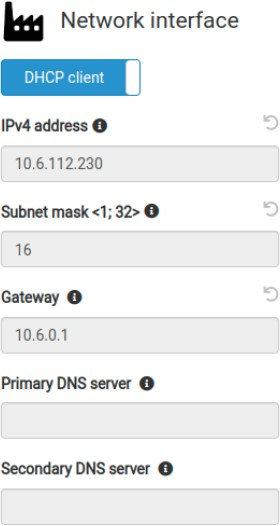
\includegraphics[width=5cm]{Thesis-report/Figures/network_interface.jpeg}
    \caption{Robot Network Interface\cite{ref2}}
    \label{fig1.Photoneo Cmaera}
\end{figure}
 As outlined in the Robot Communication, the Action Request Communication Channel helps the visual controller and the robotic controller communicate with one another.  The vision controller creates a TCP server, which the robotic controller connects to and sends requests to.
 It is advised to keep the Action Request Server port section empty and use the default port for this TCP server.  It is necessary to use the same port on the robot side when a custom port is defined \cite{ref2}.

\subsubsection{Vision Controller Interface:}
To connect the 3D sensor, gigabit Ethernet cables (Cat5e or higher category) are required.  Multiple 3D sensors can be connected using a gigabit switch.  The switch or Ethernet connection of the 3D sensor is always connected to the network of the scanner \cite{ref2}.
\begin{figure}[h]
    \centering
    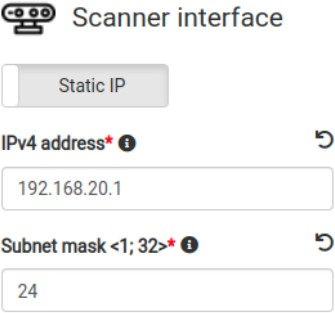
\includegraphics[width=5cm]{Thesis-report/Figures/scanner_interface.jpeg}
    \caption{Robot Network Interface \cite{ref2}}
    \label{fig1.Photoneo Cmaera}
\end{figure}

 Setting up localization settings, calibrating the robot camera, and seeing 3D scans all require a well-configured connection to the 3DSensor. To set up the network interface that the vision controller uses to connect to the Photoneo 3D Sensor, select the Scanner Interface section under the Network tab\cite{ref2}.\\

 Photoneo 3D Sensors have both a programmable IPv4 address and a fixed IPv6 link-local address. IPv6 connections are better than IPv4 ones. However, in the event that the IPv6 connection is blocked or fails, the IPv4 address is used.  It is therefore recommended to have a valid IPv4 network configuration. We use the proper IP address settings on the sensor side using the PhoXi Control program in all scenarios. The interface can be configured to run a DHCP server or to use any random static IP address\cite{ref2}.\\

\subsubsection{Communication of Robot With Vision Camera}
Communication between the vision controller and the robot controller is made possible via the robot interface on the vision controller and the robot module running on the robot controller\cite{ref2}.\\

\begin{figure}[h]
    \centering
    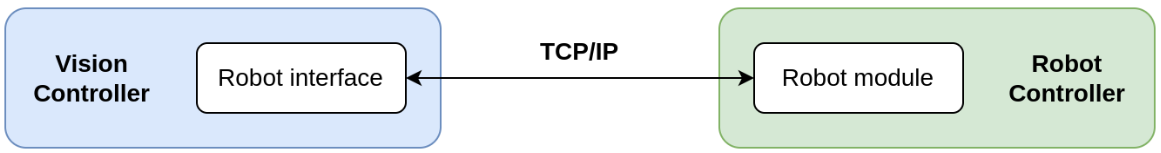
\includegraphics[width=14cm]{Thesis-report/Figures/communication.png}
    \caption{Communication with camera \cite{ref2}}
    \label{fig1.Photoneo Cmaera}
\end{figure}

The Vision Controller's scanner port is directly attached to a single Photoneo 3D sensor. 
The vision controller's network port is directly connected to a desktop PC for remote control.
The robot controller is directly attached to the vision controller's robot port\cite{ref2}.

\begin{figure}[h]
    \centering
    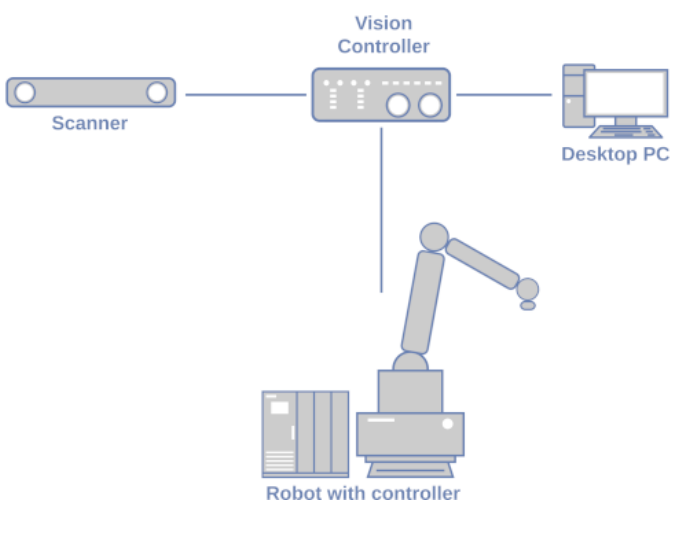
\includegraphics[width=12cm]{Thesis-report/Figures/connection.png}
    \caption{Whole camera with Robotic controller setup\cite{ref2}}
    \label{fig1.Photoneo Cmaera}
\end{figure}

\newpage
 \subsubsection{Protocol TCP/IP}
The robot controller and the vision controller communicate via the TCP/IP protocol. Network connectivity is an optional feature that some robot controllers do not come with by default\cite{ref2}.

\subsubsection{Channel of communication}
The robot module functions as a TCP client, while the vision controller establishes a TCP server. The client is called the Action Request Client, while the server is called the Action Request Server. The Action Request Client communicates with the Action Request Server over this channel. After receiving the action request, the vision controller carries it out and replies to the robotic controller\cite{ref2}.\\\\


\begin{figure}[h]
    \centering
    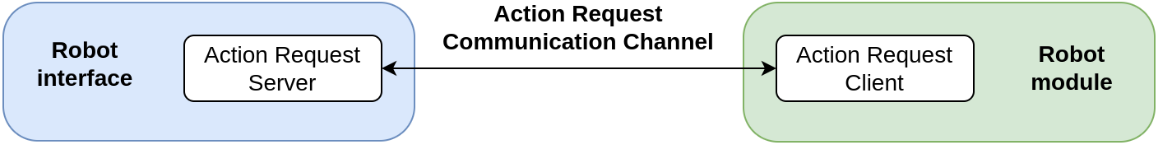
\includegraphics[width=14cm]{Thesis-report/Figures/channel.png}
    \caption{Channel Communication \cite{ref2}}
    \label{fig1.Photoneo Camera}
\end{figure}

The robot connection status is currently indicated by the following indicator:

 Action Request Client: The condition of the Action Request Server and the Action Request Client's connection via the Action Request Communication Channel. It may exist in one of two states: \cite{ref2}
 \begin{enumerate}
     \item  \textbf{CONNECTED:} Due to its connection to the Action Request Server, the Action Request Client can send requests\cite{ref2}.
      \item   \textbf{DISCONNECTED:} The Action Request Client is awaiting a fresh connection because it is not currently linked to the Action Request Server\cite{ref2}.

 \end{enumerate}

 Every vision system has a status indication that shows the current status of the connection to the related Photoneo 3D Sensor.

        Each indicator bears the identification number of the vision system to which it belongs.
  \begin{enumerate}
  \item  \textbf{CONNECTED:} The vision system's 3D sensor is connected\cite{ref2}.
  \item   \textbf{DISCONNECTED:}  There is no connection to the 3D sensor linked to vision system 2\cite{ref2}.
 \end{enumerate}

\subsubsection{Network (EC, HC)}
For the vision controller to connect with the robot and the 3D sensor, the robot interface (and robot controller IP) and the vision controller's 3D sensor interface need to be set up correctly. This is not required for marker space calibration\cite{ref2}.
\subsubsection{Vision }
It is necessary to thoroughly configure the visual system that will be calibrated. Make sure the following vision system parameters are set up correctly before beginning the calibration:
 Scanner ID: This vision system uses a 3D sensor. If the scanner interface is configured correctly, the linked 3D sensors will show up in the drop-down list of accessible 3D sensors.
The calibration space and scanner position specify the 3D sensor's mount point and, consequently, the calibration type. The scanner model is automatically calculated based on the selected 3D sensor\cite{ref2}.



%%%%%%%%%%%%%%%%%%%%%%%%%%%%%%%%%%%%%%%%%%%%%%%%%%%%%%%%%%%%%%%%%%%%%%%%%%%%%%%%%%%%%%
\subsubsection{6-Axis Cobot-Delta}
The cobot that we have used for the conveyor tracking system is a 6-axis cobot called a Delta robot. The robot mainly moves towards its target position by getting the values from the camera in the form of quaternion values\cite{ref2}.

\begin{figure}[H]
  \centering
  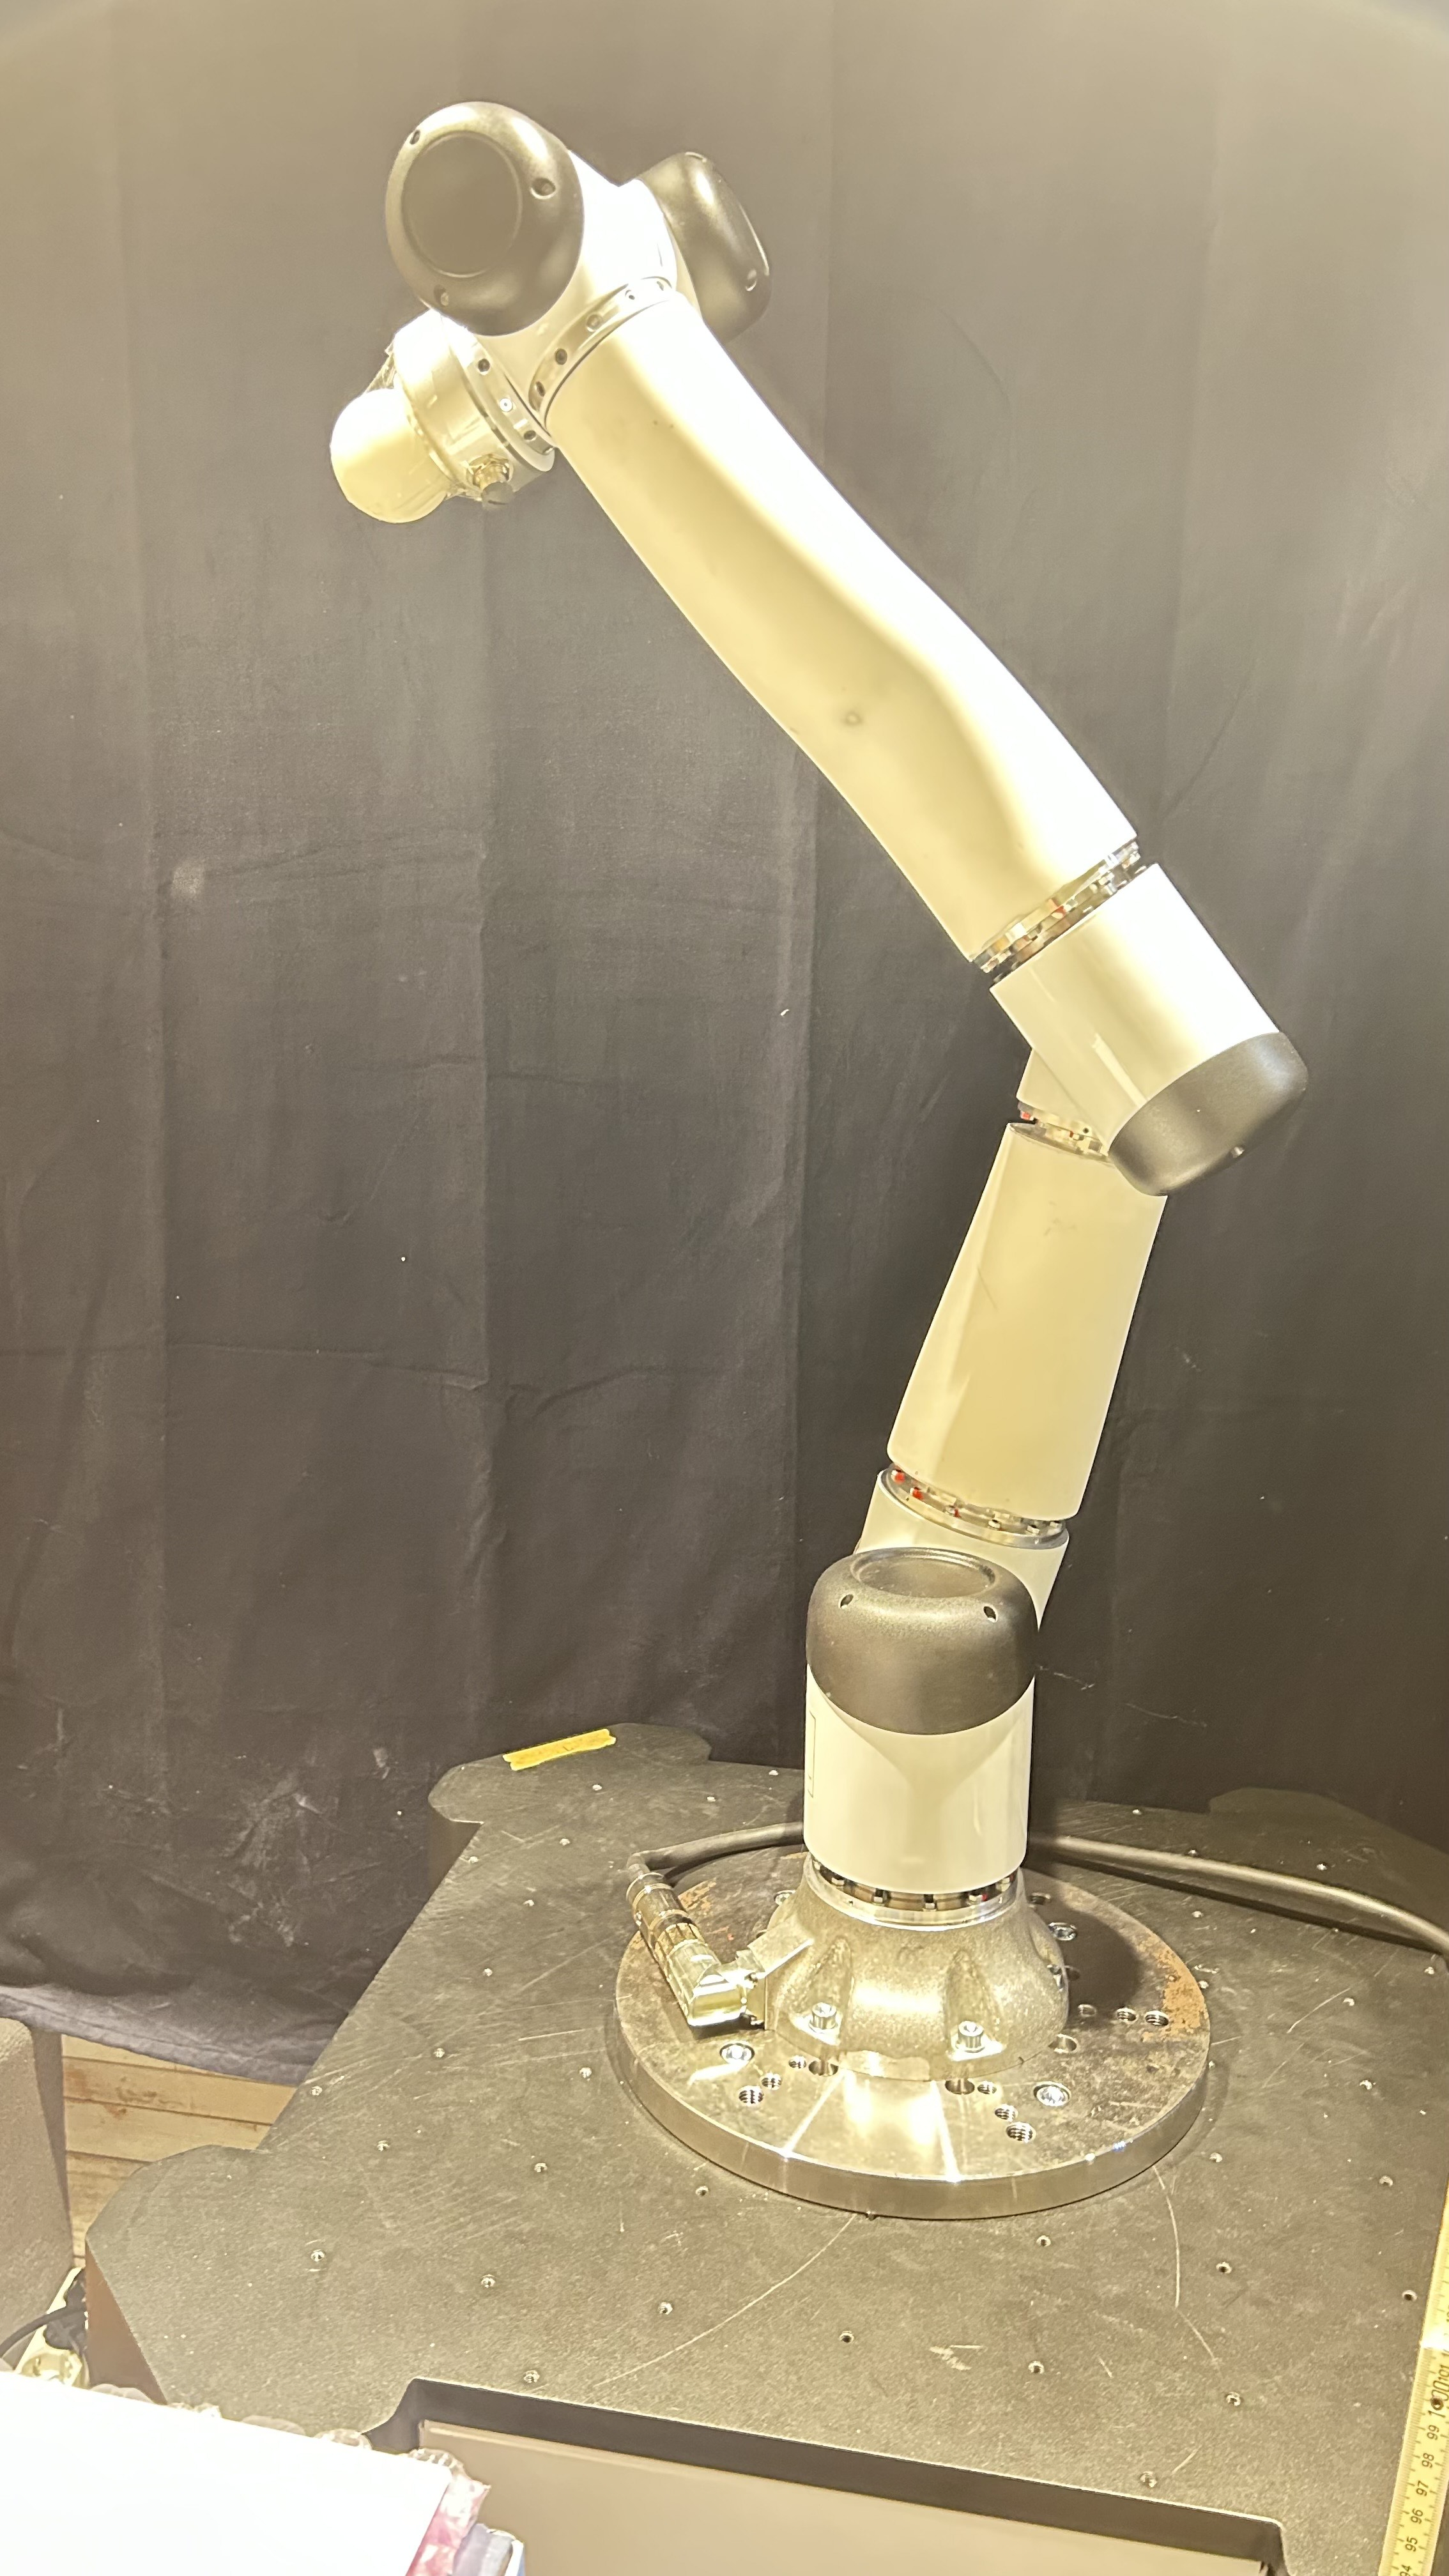
\includegraphics[width=3.5cm]{Thesis-report/Figures/robot.jpeg}
  \caption{Delta Robot}
  \label{fig:delta_robot}
\end{figure}


\subsubsection{RobotiQ 140 Gripper}
The RobotiQ 140 gripper is a two-finger gripper that mainly works under the principle of Modbus communication. Its 85 mm stroke, 230 N max gripping force, and 5 kg max payload make it ideal for low-volume, high-changeover settings.

\begin{figure}[H]
  \centering
  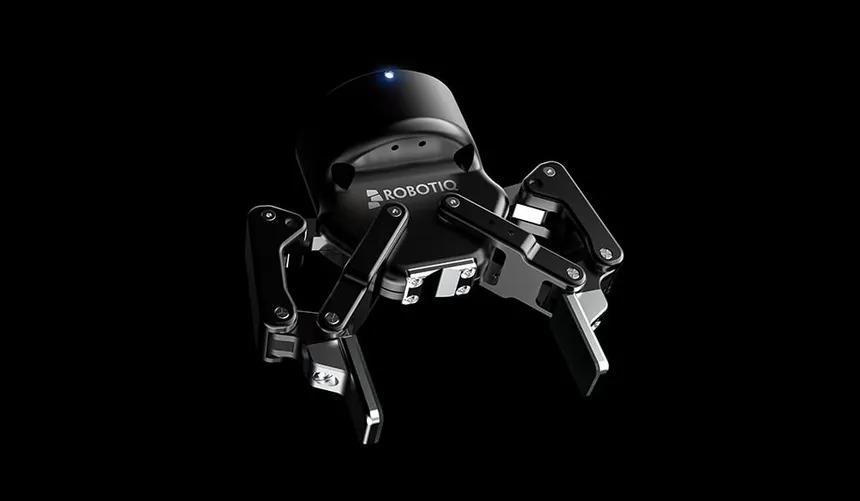
\includegraphics[width=7cm]{Thesis-report/Figures/cobot_gripper_2F_85-ezgif.com-webp-to-jpg-converter.jpg}
  \caption{RobotiQ 140 Gripper\cite{ref26}}
  \label{fig:robotiq_140}
\end{figure}

\subsection{3D Scanning}
The act of gathering data from an object's surface and turning it into data points is known as 3D scanning. These data points are utilized for a digital replication of the scanned object or for a dimension analysis\cite{ref17}.\\

\subsection{Types of 3D scanning}

\subsubsection {Laser Scanning}
Two devices are often used in laser scanning; one directs a laser beam onto a surface, and the other records the precise spot where the object contacts the beam. The angle of reflection and the distance between the surface and the scanner can be determined via triangulation.  Time of flight measurement, structured light scanning, stereophoto-grammetry, laser interferometry, and many other techniques are comparable to the Train-gulation method\cite{ref17}.

\subsubsection {Structure Light Scanning}
This technology projects structured light patterns, such as simple geometric patterns or parallel lines, onto a surface.  The object's shape will cause the patterns to distort.  It is feasible to rebuild the scanned surface using a camera to analyze these deformations, distinguish edges, and determine the separation between the item and the scanner \cite{ref17}.

\subsection {Photogrammetry}
Triangulation is used in photogrammetry to intersect particular points within 2D images based on the angles at which those points can be found. The size, quantity, and quality of the item's images all have a big impact on creating an appropriate 3D model\cite{ref17}. 

\subsection{Time fo Flight}
The time of flight is a measure of how long it takes light to move from an illumination source to a scene and back. The main barrier in this case is the speed of light itself.  Time is typically measured using a modulated signal's phase shift. High pixel modulation frequencies must be used to achieve a respectable level of depth accuracy. The primary drawback in this case is physics, since a greater frequency results in less charge transfer, which lowers contrast and Signal‑to‑Noise Ratio. The restriction suggests an accuracy level that ToF systems can achieve. Usually, it falls within the centimeter range. Another issue is interreflections, which can significantly bend the surface\cite{ref15}.

\subsection{Active stereo}
By projecting a synthetic texture onto an object, active stereo addresses the unreliable passive stereo. Nevertheless, it still has to resolve the computationally demanding picture correspondence matching problem. Because of the complexity of the matching problem, the projected texture can be either high frequency, which can satisfy a higher resolution but usually has poor reliability, or low frequency, which typically uses random laser dots and can provide higher reliability but poor resolution (the features 15 are sparse)\cite{ref15}.

\subsection{Structured patterns/dots}
A spatially encoded pattern is used in structured patterns/dots technology to encode depth disparity information into pattern patches, which are usually projected through a laser diffraction grating in the form of a carefully planned dot collection. The camera needs to be able to see enough of the patch in order to properly record the depth information and reconstruct the code. This produces artifacts on the surfaces' edges and tiny objects. To reconstitute individual dots in the projection (and hence 3D measurements), the Nyquist-Shannon theorem necessitates an order of magnitude better camera resolution. Modern systems use about 25 camera pixels for each 3D measurement, producing about 70k 3D points \cite{ref15}. 

\subsection{Parallel Structured Light}

Parallel Structured Light parallelizes the sequential structured light using a sophisticated sensor design, which enables it to record the scene illuminated by various patterns. In addition to sharing many of the sequential structured light's benefits, such as resolution and accuracy, it also overcomes one of its main drawbacks: the inability to capture a dynamic environment. Photoneo's Parallel Structured Light gets around the restriction by projecting and capturing numerous encoded patterns. Pixel modulations within our proprietary CMOS sensor are used to accomplish this. Multiple groups of separately modified pixels make up the sensor itself \cite{ref15}.  \\


The Parallel Structured Light's main advantages are:
\begin{enumerate}
 \item  Rapid motion scanning: 40 m/s motion is achieved with single frame acquisition \cite{ref15}.
\item A more effective depth coding method with accurate, per-pixel measurement that offers ten times greater resolution and accuracy than rival technologies\cite{ref15}
 \item No motion blur: exposure time of 10 µs per pixel\cite{ref15}
 \item Quick capture of 1068 x 800 point clouds at 60 frames per second\cite{ref15}
\item Patent-pending active ambient light rejection technology for outdoor use in direct sunlight\cite{ref15}
 \item Active rejection of ambient light through interreflection suppression\cite{ref15}
\item Several devices using the same space at the same time\cite{ref15}\\
\end{enumerate}

A control unit that operates in tandem with the projection is in charge of these groups. The coded patterns are inserted into the groups rather than changing the projection itself. The coded patterns injected at the end of the frame may cause the sensor to produce more than 20 different virtual representations of the scene.  Any pattern commonly used for sequential structured light can be utilized to adapt the universal approach on the fly to suit different materials and light sources\cite{ref15}. \\

After undergoing embedded processing, these virtual images are sent via gigabit Ethernet to a client PC.  Three types of outputs are provided by the sensor: \cite{ref15}
\begin{enumerate}
    \item Point Cloud: 32 bits per channel  XYZ \cite{ref15}
    \item 32 bits per channel is the normal map.  XYZ \cite{ref15}
    \item Texture: Grayscale, 10/12 bits \cite{ref15}
\end{enumerate}

The sensor produces outputs with a resolution of 1068 x 800 when in "one frame" camera mode.  Approximately 500k individual measurements were used to interpolate these positions. The typical z-noise standard deviation at a distance of one meter is less than 0.5 mm (key advantage 1).  Because of the pixel design, each photon makes the best possible contribution to the 3D measurement.  The technology surpasses its rivals and offers the best XYZ resolution thanks to sub-pixel accuracy coding (high z-precision) and an efficiency of just 4.5 pixels per 3D measurement (benefit 2)\cite{ref15}. \\

The "scanner mode," which is designed for still photos, is the alternate operating mode.
 The sensor's raw sensoric output in this mode is 1602 × 1200 individual measurements. This is recorded in three consecutive frames. A laser that has been deflected by a mirror illuminates the scene.  The projection's 10 µs per pixel exposure may guarantee constant, motion-blur-free data (benefit 4)\cite{ref15}.


\subsection{Vision Controller}
The figure 3 below shows the vision controller connected to the Photoneo camera and the robotic controller using Ethernet (IPV4 address).
\begin{figure}[h]
    \centering
    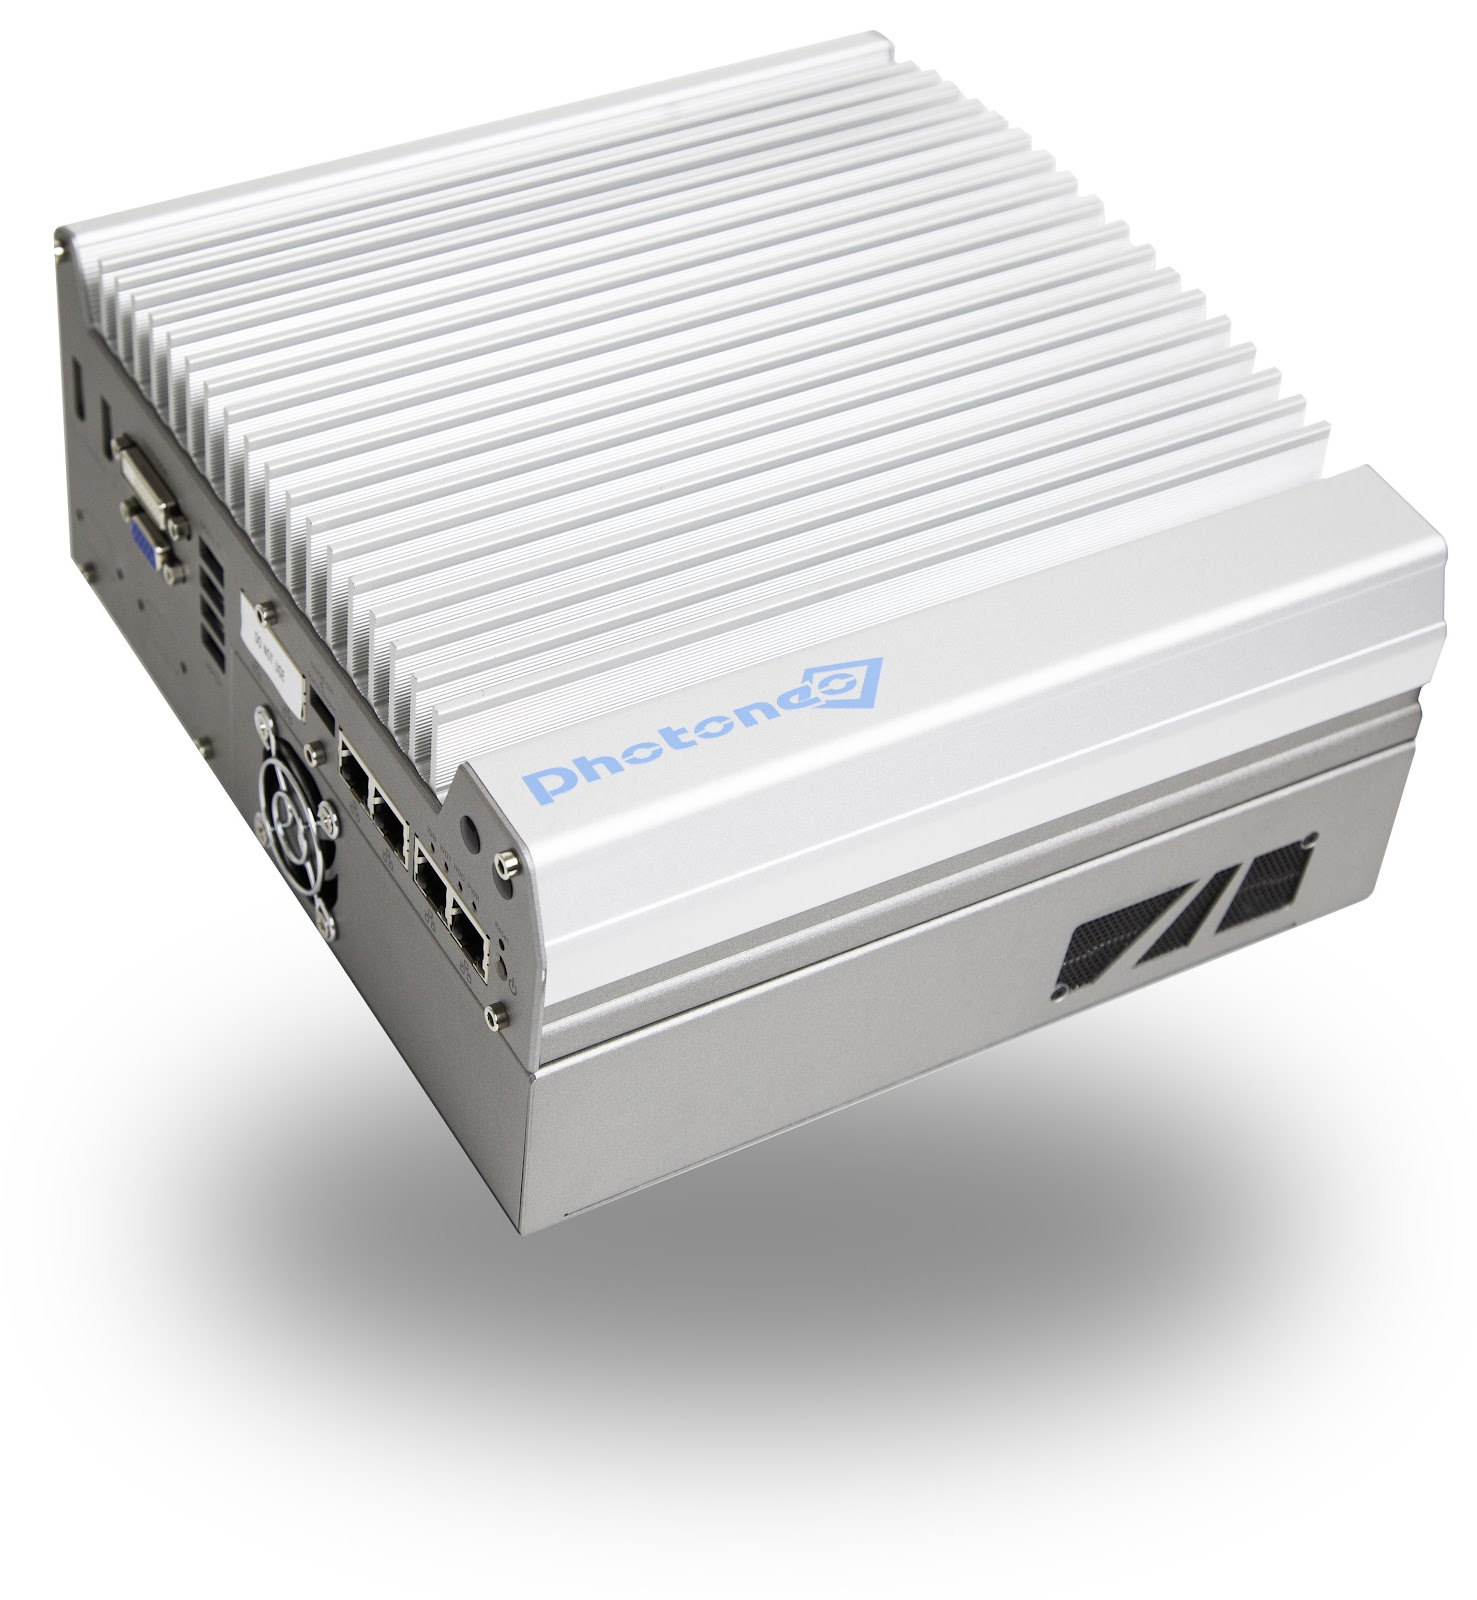
\includegraphics[width=4cm]{Thesis-report/Figures/vision controller.png}
    \caption{Vision Controller \cite{ref2}}
    \label{fig1.Photoneo Cmaera}
\end{figure}
The vision controller is connected to a PC through the web interface to trigger the camera and see the Web interface for communication.To connect the 3D sensor, gigabit Ethernet connections of Cat5e or above are needed.  Multiple 3D sensors can be connected using a gigabit switch.  Multiple 3D sensors can be connected using a gigabit switch. The Ethernet connection from the switch or 3D sensor is linked to the scanner's physical network port in both scenarios. To visualize 3D scans, calibrate robot cameras, and establish localization settings, a connection to the 3D sensor is required.To set up the network interface that the vision controller uses to connect to the Photoneo 3D sensor(s), enter the Network page and select the Scanner Interface section. Both a fixed IPv6 link-local address and a programmable IPv4 address are features of Photoneo 3D sensors.\cite{ref15}
\newpage
\subsection{Marker Pattern}\\
\begin{figure}[h]
    \centering
    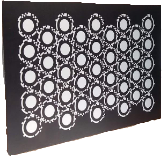
\includegraphics[width=4cm]{Thesis-report/Figures/marker_pattern.png}
    \caption{Marker Pattern} \cite{ref2}
    \label{fig1.Photoneo Cmaera}
\end{figure}
Figure 4 above shows the S30 calibration board that helps calibrate the conveyor belt, which aligns the coordinates of the object with the conveyor belt for objects passing through the belt. To enable the robot to retrieve objects from the moving conveyor belt, the belt can be used to align the object coordinates with the conveyor belt\cite{ref2}.
%%%%%%%%%%%%%%%%%%%%%%%%%%%%%%%%%%%%%%%%%%%%%%%%%%%%%%%%%%%%%%%%%%%%%%%%%%%%%%%%%%%%%%
\newpage
\printbibliography
\end{document}
